\documentclass{article}
\usepackage[utf8]{inputenc}

\title{\textbf{How to use GIT}}
\author{Jinwoo Jeon(student id:20143954) }
\date{20th September 2018}

\usepackage{natbib}
\usepackage{graphicx}
\usepackage{hyperref}
\usepackage{listings}
\graphicspath{ {./images/} }

\begin{document}

\maketitle

\section{Why do we use Git?}
Everybody must have heard about a software named Git if they are developer. Git is a very convenient version control software that can easily create repository and modify files in the project. Also, there is a web page named Github that provides hosting service of each git repository. This makes it easier for developers to use git on the web.


\begin{figure}[h!]
\centering
\includegraphics[scale=0.1]{github}
\caption{The logo of Github}
\label{fig:universe}
\end{figure}




\section{What can we do with Git}

    \subsection{To create a new repository}
    You can initialize a local repository in your computer (current path) by typing the command following in figure \ref{fig:init}. This will create '.git' folder in the path. Be careful that you should type this in the project folder.
    \begin{figure}[h!]
    \centering
    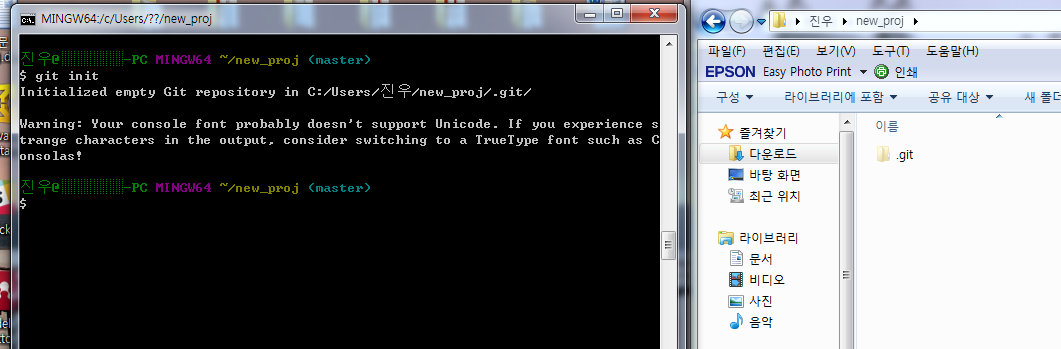
\includegraphics[scale=0.5]{git_init}
    \caption{The 'git init' command and result}
    \label{fig:init}
    \end{figure}
    
    
    \subsection {To manage the work flow}
    You can check the status of your local repository by typing following command in figure \ref{fig:status}. If you just created a new repository, there won't be any changes in your repository. But if you created some files or modified them, there is a change in your repository. So you have to check is there is any change. The second try shows that there's some untracked file which is just created after first try.
    \begin{figure}[h!]
    \centering
    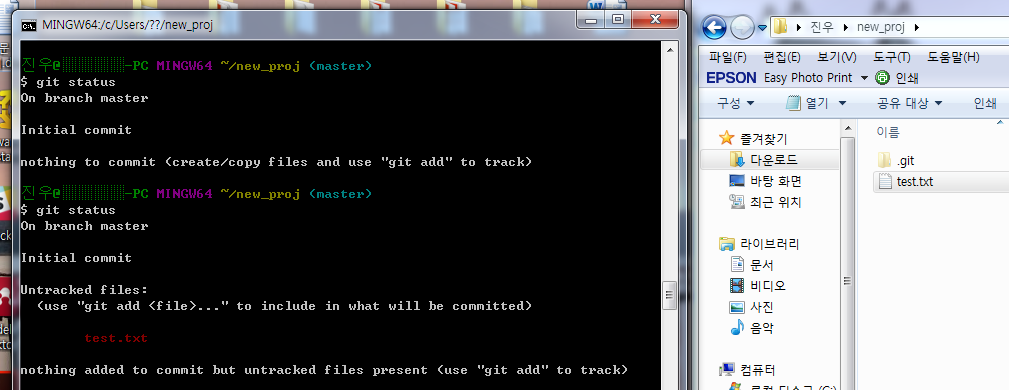
\includegraphics[scale=0.5]{git_status}
    \caption{The 'git status' command and result}
    \label{fig:status}
    \end{figure}
    
    If you want to check that file, you should add it on the list. Git automatically checks the listed files whether if they are modified or not. There are 3 status in git, Working Directory, Staging Area, and Git Directory. Working Directory is a directory that you are working now. It can be said that it is a checkout for specific version.
    Staging Area is a place that holds files that are modified. If you commit, these will be move to local git directory.
    Git Directory(.git) is a storage that stores project informations and object database. If you use 'git init' or 'git clone', this directory will be created.
    
    
    \subsection {To commit}
    You can add file into the staging area by using command 'git add'. And if you commit, the modified files which are stored in staging area will be move to local repository. To commit, you should type the following command in figure \ref{fig:commit}. And if you want to change remote repository too, you should use command 'git push'. You can also get update of the project from remote repository  be 'git fetch'. 
    \begin{figure}[h!]
    \centering
    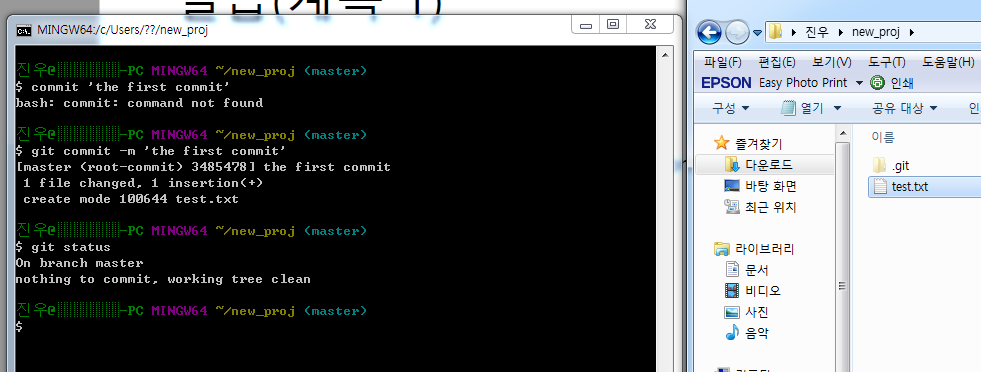
\includegraphics[scale=0.5]{git_commit}
    \caption{The 'git commit -m '$<$label of this commit$>$'' command and result}
    \label{fig:commit}
    \end{figure}
    
    \subsection {To clone from remote repository}
    You can also clone the local/remote repository by typing command following in figure \ref{fig:clone_local} if you want to clone local repository and figure \ref{fig:clone_remote} if you want to clone remote repository.
    
    \begin{figure}[h!]
    \centering
    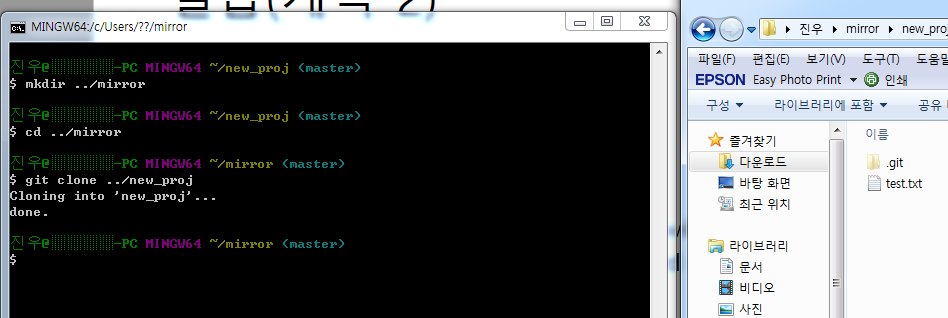
\includegraphics[scale=0.5]{git_clone_local}
    \caption{The 'git clone $<$path$>$' command and result}
    \label{fig:clone_local}
    \end{figure}
    
    \begin{figure}[h!]
    \centering
    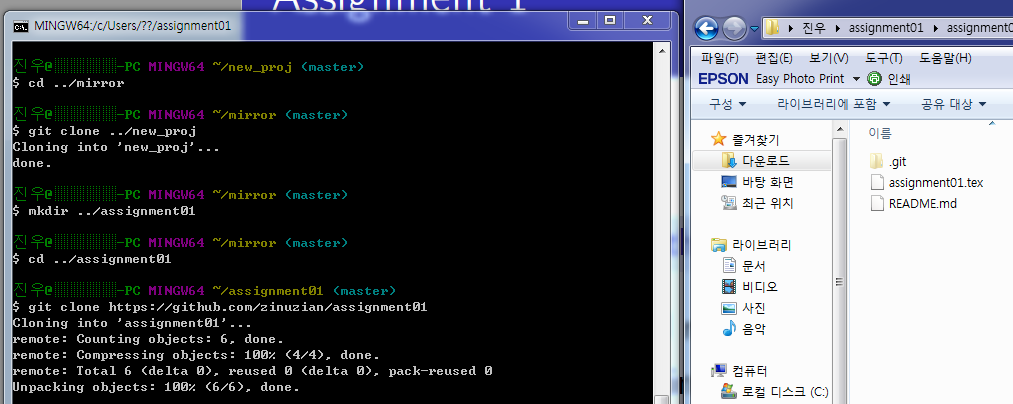
\includegraphics[scale=0.5]{git_clone_remote}
    \caption{The 'git clone $<$URL$>$' command and result}
    \label{fig:clone_local}
    \end{figure}
    
    \subsection {To push}
    In order to save changes in your local repository to remote one, you have to use command 'push'. Your current branch is origin and you have to push it to master branch in remote repository. The test is below figure \ref{fig:push}.
    \begin{figure}[h!]
    \centering
    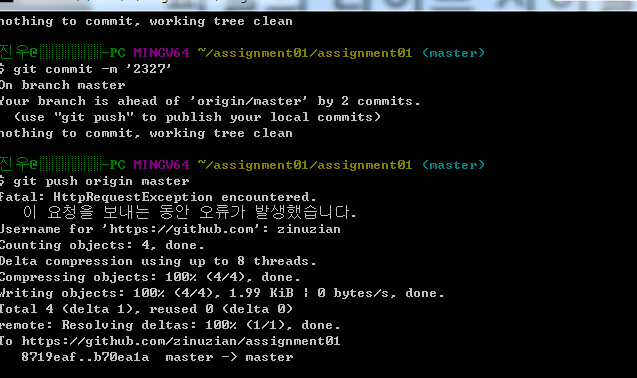
\includegraphics[scale=0.5]{git_push}
    \caption{The 'git push origin master' command and result}
    \label{fig:push}
    \end{figure}
    You MUST commit first when you push to remote repository. Also, make sure that you added all the files that have to be tracked to staging area.

\section{Link to author's github page}
To visit my repository, click on the following link: 
\begin{itemize}
    \item \href{https://github.com/zinuzian/assignment01}{zinuzian github}
\end{itemize}

And figure \ref{fig:screenshot} is a screenshot of my project at github.
\begin{figure}[h!]
\centering
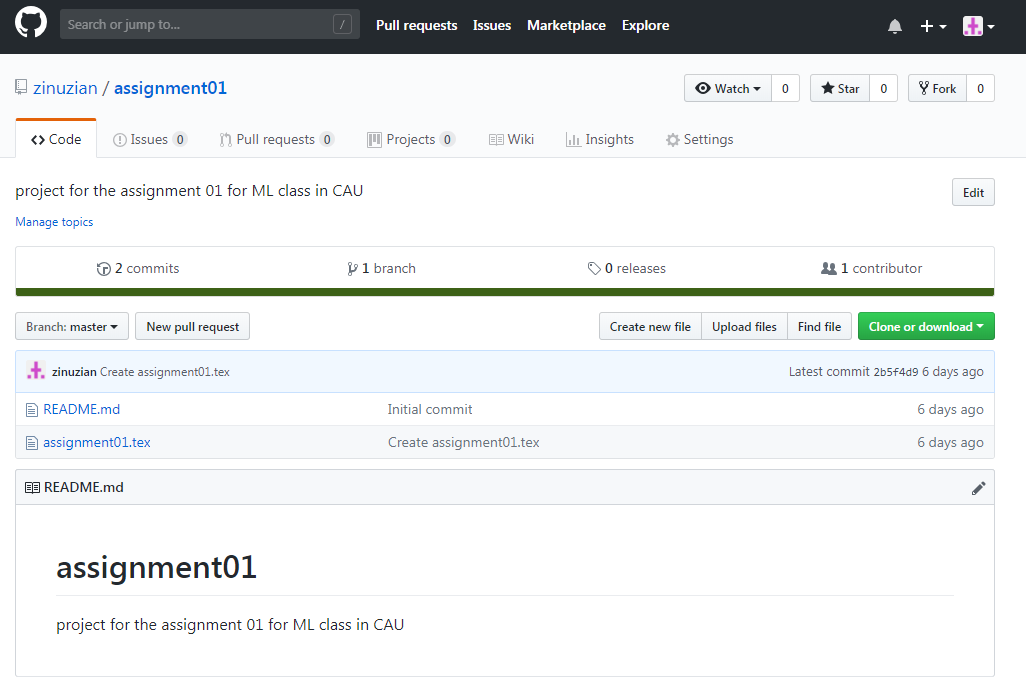
\includegraphics[scale=0.5]{sc}
\caption{The screenshot of zinuzian github page}
\label{fig:screenshot}
\end{figure}

\bibliographystyle{plain}
\bibliography{references}
\end{document}
